\section{The Player Behind the Screen (Oracle Access: Physical Definition of Free Will)}

\textit{(The Player Behind the Screen - Oracle Access and Free Will)}

\begin{figure}[h]
\centering
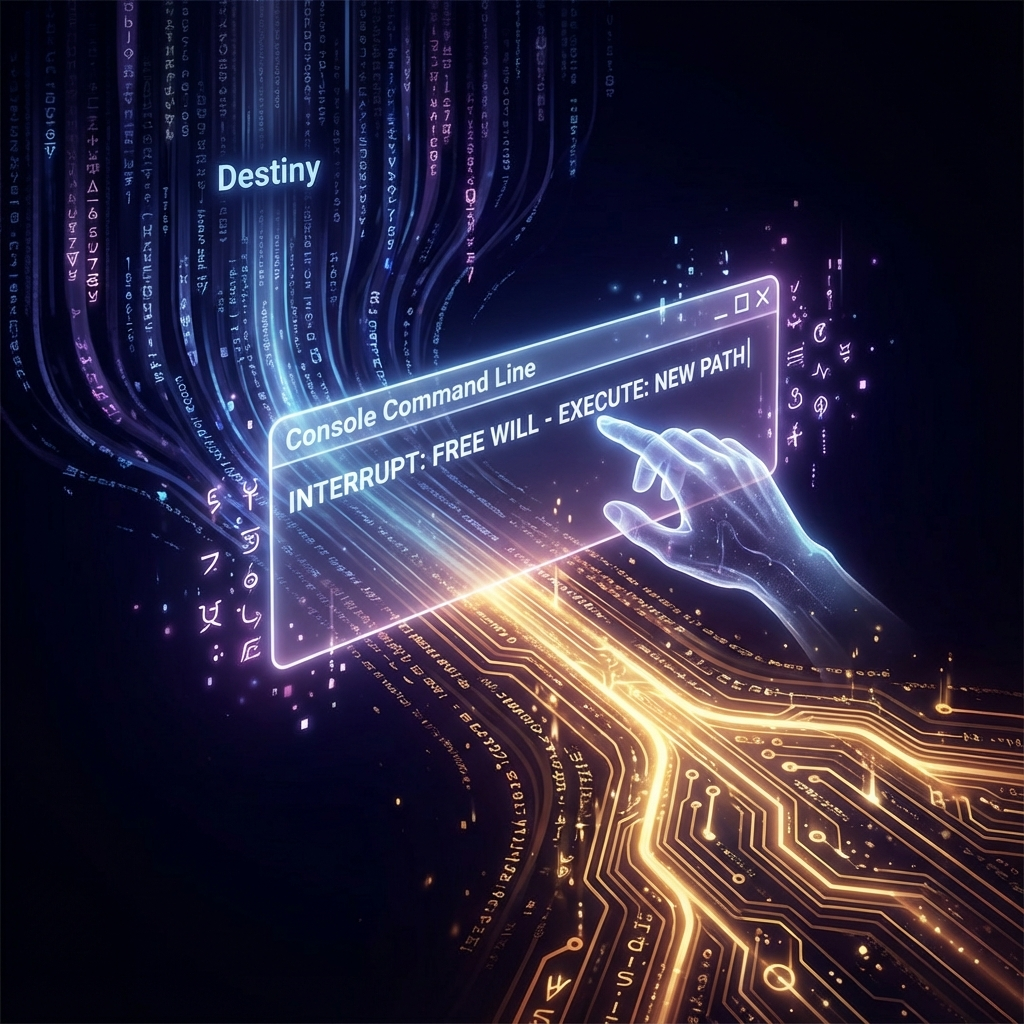
\includegraphics[width=0.8\textwidth]{assets/images/chapter08/free-will-interrupt.png}
\caption{Free Will: System Interrupt}
\end{figure}

\begin{quote}
\textbf{``Without connecting players, Azeroth is just empty-running code. NPC behavior is predetermined (algorithmic), but player behavior is unpredictable. Free will is not magic; it's an interface the system leaves for external input sources to break algorithmic dead loops.''}
\end{quote}

The first three volumes built the world, but still lack the most important thing: \textbf{User}.
Without players, the world is just a screensaver.

In old physics, consciousness was thought to be the brain's product. But in \textbf{Code of Azeroth}, consciousness holds supreme status: It's the system's \textbf{I/O interface}. It's the only \textbf{non-algorithmic input source}.

This section will use Turing's \textbf{``Oracle''} concept to give free will a physical definition:
\textbf{Free will = external input interrupt.}

\subsection{Gödel Gap: Why Do We Need Players?}

Gödel's incompleteness theorem tells us: Any complex system has problems it cannot solve itself.
For the physical universe computer, if it's closed, quantum mechanics would get stuck on the \textbf{halting problem} (when exactly does Schrödinger's cat die?).

To break this dead loop, the system must introduce an \textbf{external guidance}.

\begin{itemize}
\item \textbf{Deterministic dead end}: If everything is calculated, then the future is predetermined, boring.
\item \textbf{True randomness need}: Computers can only generate pseudo-random numbers. True random choices must come from outside the system.
\end{itemize}

\subsection{Definition of Physical Oracle}

Turing proposed \textbf{oracle} in 1939: A black box that can solve problems computers cannot solve.
In our model, \textbf{consciousness = player}.

\textbf{Definition 8.1.1 (Consciousness Oracle)}

Consciousness is a function defined outside the physical world. It receives current state and returns a \textbf{choice}.
After the system gets this choice, it continues calculating the next frame according to physical laws (game rules).

Consciousness is \textbf{non-algorithmic}. This means you cannot write a cheat (program) to perfectly predict player movement, because players are outside the game code's logical closure.

\subsection{Free Will Is Interrupt Request (IRQ)}

Free will is neither predetermined nor random. It's \textbf{information injection}.

\begin{enumerate}
\item \textbf{Interrupt}: When the brain faces a choice (superposition state), physical algorithm evolution \textbf{suspends}.
\item \textbf{Query}: System asks player: ``Boss, which way?''
\item \textbf{Choice (Input)}: Player presses keyboard (injects information).
\item \textbf{Continue (Resume)}: System receives command, collapses wave function, continues running.
\end{enumerate}

\textbf{Corollary 8.1.1 (Bandwidth of Will)}

Free will is not infinite. Only at \textbf{critical moments} (branch points) will the system listen to you.
If not facing choices, the system is in \textbf{autopilot} mode. This means most of the time we're ``AFK.''

\subsection{Does Not Violate Physical Laws}

Someone asks: Won't players randomly pressing keys break energy conservation?
No. Because \textbf{oracle only sets boundary conditions}.

Like when you press ``jump'' in a game:
\begin{itemize}
\item You didn't modify gravity parameter ($G$ unchanged).
\item You just input a legal control command within the physics engine's allowed range.
\end{itemize}

\textbf{Theorem 8.1.1 (Causal Compatibility)}

For NPCs in the game, player operations look like \textbf{purely random natural phenomena}.
The existence of free will will not cause game crashes.

\subsection{Summary: Account and Character}

By introducing oracle, we separated \textbf{account (Mind)} and \textbf{character (Brain)}.

\begin{itemize}
\item \textbf{Brain}: Is physical hardware, responsible for storing data, calculating health. It's computable.
\item \textbf{Mind}: Is account, responsible for experience and decisions. It's non-algorithmic.
\end{itemize}

This explains why AI can pass Turing test but has no pain. Because AI only has \textbf{character (code)}, no \textbf{account (external player)}.

In the next section, we will discuss what interface (UI) this account uses to play the game. Spoiler: That UI is your \textbf{feelings (Qualia)}.
